\documentclass[tikz,border=5pt]{standalone}
\usepackage{amsmath}
\usetikzlibrary{arrows.meta,positioning,calc}

\definecolor{arrowgray}{HTML}{333333}
\definecolor{inputfill}{HTML}{EAF1F8}
\definecolor{inputborder}{HTML}{4A6B8A}
\definecolor{baselinefill}{HTML}{FBEBD9}
\definecolor{baselineborder}{HTML}{B8702E}
\definecolor{residualfill}{HTML}{E4F2E7}
\definecolor{residualborder}{HTML}{3C7A4A}
\definecolor{correctionfill}{HTML}{EDE4F5}
\definecolor{correctionborder}{HTML}{6A4C93}
\definecolor{predictionfill}{HTML}{E3EEF9}
\definecolor{predictionborder}{HTML}{2F5F8A}
\definecolor{evaluationfill}{HTML}{F2F2F2}
\definecolor{evaluationborder}{HTML}{7F7F7F}

\begin{document}
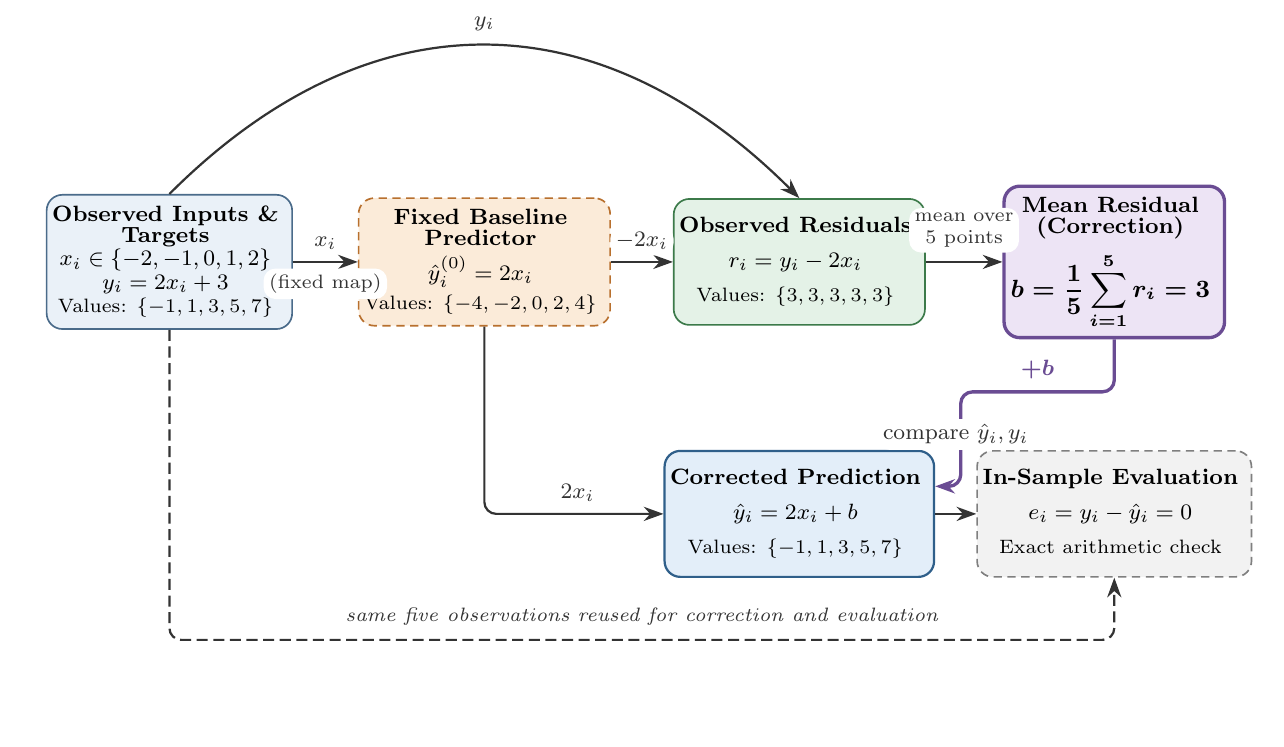
\begin{tikzpicture}[
  x=1cm,y=1cm,
  common/.style={
    rectangle,
    rounded corners=2mm,
    line width=0.6pt,
    minimum height=1.4cm,
    align=center,
    text depth=0.25ex,
    text height=1.2ex,
    font=\footnotesize
  },
  block/.style={
    common,
    minimum width=2.8cm,
    minimum height=1.6cm,
    inner xsep=2pt,
    inner ysep=3pt,
    text height=,
    text depth=
  },
  flow/.style={
    -{Stealth[length=2.5mm,width=1.8mm]},
    line width=0.8pt,
    draw=arrowgray,
    rounded corners=1.5mm
  },
  labeltext/.style={
    font=\footnotesize,
    text=arrowgray,
    fill=white,
    inner sep=2pt,
    align=center
  }
]

% Borderless white canvas, approximately 16:9.
\path[use as bounding box] (0,-0.2) rectangle (15.6,8.575);
\fill[white] (0,-0.2) rectangle (15.6,8.575);

\node[block,fill=inputfill,draw=inputborder]
  (inputs) at (1.8,5.6) {%
    \begin{tabular}{@{}c@{}}
      \textbf{Observed Inputs \&}\\[-2pt]
      \textbf{Targets}\\[-1pt]
      $x_i\in\{-2,-1,0,1,2\}$\\[-1pt]
      $y_i=2x_i+3$\\[-1pt]
      {\scriptsize Values: $\{-1,1,3,5,7\}$}
    \end{tabular}
  };

\node[
  block,
  fill=baselinefill,
  draw=baselineborder,
  dash pattern=on 3pt off 2pt
] (baseline) at (5.8,5.6) {%
    \begin{tabular}{@{}c@{}}
      \textbf{Fixed Baseline}\\[-2pt]
      \textbf{Predictor}\\[1pt]
      $\hat{y}^{(0)}_i=2x_i$\\[1pt]
      {\scriptsize Values: $\{-4,-2,0,2,4\}$}
    \end{tabular}
  };

\node[block,fill=residualfill,draw=residualborder]
  (residuals) at (9.8,5.6) {%
    \begin{tabular}{@{}c@{}}
      \textbf{Observed Residuals}\\[3pt]
      $r_i=y_i-2x_i$\\[3pt]
      {\scriptsize Values: $\{3,3,3,3,3\}$}
    \end{tabular}
  };

\node[
  block,
  fill=correctionfill,
  draw=correctionborder,
  line width=1.2pt
] (correction) at (13.8,5.6) {%
    \begin{tabular}{@{}c@{}}
      \textbf{Mean Residual}\\[-2pt]
      \textbf{(Correction)}\\[4pt]
      {\small $\displaystyle
        \boldsymbol{b=\frac{1}{5}\sum_{i=1}^{5}r_i=3}$}
    \end{tabular}
  };

\node[
  block,
  minimum width=3.2cm,
  fill=predictionfill,
  draw=predictionborder,
  line width=0.8pt
] (prediction) at (9.8,2.4) {%
    \begin{tabular}{@{}c@{}}
      \textbf{Corrected Prediction}\\[3pt]
      $\hat{y}_i=2x_i+b$\\[3pt]
      {\scriptsize Values: $\{-1,1,3,5,7\}$}
    \end{tabular}
  };

\node[
  block,
  fill=evaluationfill,
  draw=evaluationborder,
  dash pattern=on 3pt off 2pt
] (evaluation) at (13.8,2.4) {%
    \begin{tabular}{@{}c@{}}
      \textbf{In-Sample Evaluation}\\[3pt]
      $e_i=y_i-\hat{y}_i=0$\\[3pt]
      {\scriptsize Exact arithmetic check}
    \end{tabular}
  };

% Inputs and fixed baseline.
\draw[flow]
  (inputs.east) --
  node[labeltext,above=2pt] {$x_i$}
  node[labeltext,below=2pt,font=\scriptsize] {(fixed map)}
  (baseline.west);

% Direct target feed, clear of the baseline.
\draw[flow]
  (inputs.north)
  to[out=45,in=135,looseness=1.15]
  node[labeltext,above=3pt,pos=0.5] {$y_i$}
  (residuals.north);

\draw[flow]
  (baseline.east) --
  node[labeltext,above=2pt] {$-2x_i$}
  (residuals.west);

\draw[flow]
  (residuals.east) --
  node[
    labeltext,
    above=3pt,
    font=\scriptsize
  ] {\shortstack{mean over\\5 points}}
  (correction.west);

% Baseline contribution to the corrected prediction.
\draw[flow]
  (baseline.south) |-
  node[labeltext,above=2pt,pos=0.76] {$2x_i$}
  (prediction.west);

% Separate right-edge ports keep correction and comparison arrows distinct.
\coordinate (correctionentry)
  at ($(prediction.east)+(0,0.35)$);

\draw[
  flow,
  draw=correctionborder,
  line width=1.2pt
]
  (correction.south) --
  (13.8,3.95) --
  node[
    labeltext,
    above=2pt,
    text=correctionborder
  ] {$\boldsymbol{+b}$}
  (11.85,3.95) --
  (11.85,2.75) --
  (correctionentry);

\draw[flow]
  (prediction.east) --
  node[labeltext,above=8mm]
    {compare $\hat{y}_i,y_i$}
  (evaluation.west);

% The same observations are reused for correction and evaluation.
\draw[
  flow,
  dash pattern=on 4pt off 2pt
]
  (inputs.south) --
  (1.8,0.8) --
  node[
    labeltext,
    above=3pt,
    font=\scriptsize\itshape,
    pos=0.5
  ] {same five observations reused for correction and evaluation}
  (13.8,0.8) --
  (evaluation.south);

\end{tikzpicture}
\end{document}